%%
%% Iris Liu
%% CS446 Advanced Computational Modeling
%% Agent-based Mutualism in Space
%% Manuscript Draft
%% October 31, 2020
%%

%% ---------------------------------------------
%% Copyright 2007, 2008, 2009 Elsevier Ltd
%%
%% This file is part of the 'Elsarticle Bundle'.
%% ---------------------------------------------
%%
%% It may be distributed under the conditions of the LaTeX Project Public
%% License, either version 1.2 of this license or (at your option) any
%% later version.  The latest version of this license is in
%%    http://www.latex-project.org/lppl.txt
%% and version 1.2 or later is part of all distributions of LaTeX
%% version 1999/12/01 or later.
%%
%%
\documentclass[3p,,preprint,12pt]{elsarticle}
\makeatletter\if@twocolumn\PassOptionsToPackage{switch}{lineno}\else\fi\makeatother


\usepackage{tabulary,xcolor}
\usepackage{amsfonts,amsmath,amssymb}
\usepackage[T1]{fontenc}
\makeatletter
\let\save@ps@pprintTitle\ps@pprintTitle
\def\ps@pprintTitle{\save@ps@pprintTitle\gdef\@oddfoot{\footnotesize\itshape \null\hfill\today}}
\def\hlinewd#1{%
  \noalign{\ifnum0=`}\fi\hrule \@height #1%
  \futurelet\reserved@a\@xhline}
\def\tbltoprule{\hlinewd{.8pt}\\[-12pt]}
\def\tblbottomrule{\noalign{\vspace*{6pt}}\hline\noalign{\vspace*{2pt}}}
\def\tblmidrule{\noalign{\vspace*{6pt}}\hline\noalign{\vspace*{2pt}}}
\AtBeginDocument{\ifNAT@numbers \biboptions{sort&compress}\fi}
\makeatother

  \renewenvironment{abstract}{\global\setbox\absbox=\vbox\bgroup
    \hsize=\textwidth\def\baselinestretch{1}%
  \noindent\unskip\textbf{}
   \par\medskip\noindent\unskip\ignorespaces}
   {\egroup}
  
\usepackage{ifluatex}
\ifluatex
\usepackage{fontspec}
\defaultfontfeatures{Ligatures=TeX}
\usepackage[]{unicode-math}
\unimathsetup{math-style=TeX}
\else 
\usepackage[utf8]{inputenc}
\fi 
\ifluatex\else\usepackage{stmaryrd}\fi

%% ---------------------------------------------  
% Following additional macros are required to function some 
% functions which are not available in the class used.
%% ---------------------------------------------
\usepackage{url,multirow,morefloats,floatflt,cancel,tfrupee}
\makeatletter

\AtBeginDocument{\@ifpackageloaded{textcomp}{}{\usepackage{textcomp}}}
\makeatother
\usepackage{colortbl}
\usepackage{xcolor}
\usepackage{pifont}
\usepackage[nointegrals]{wasysym}
\urlstyle{rm}
\makeatletter

%%%For Table column width calculation.
\def\mcWidth#1{\csname TY@F#1\endcsname+\tabcolsep}

%%Hacking center and right align for table
\def\cAlignHack{\rightskip\@flushglue\leftskip\@flushglue\parindent\z@\parfillskip\z@skip}
\def\rAlignHack{\rightskip\z@skip\leftskip\@flushglue \parindent\z@\parfillskip\z@skip}

%Etal definition in references
\@ifundefined{etal}{\def\etal{\textit{et~al}}}{}


%\if@twocolumn\usepackage{dblfloatfix}\fi
\usepackage{ifxetex}
\ifxetex\else\if@twocolumn\@ifpackageloaded{stfloats}{}{\usepackage{dblfloatfix}}\fi\fi

\AtBeginDocument{
\expandafter\ifx\csname eqalign\endcsname\relax
\def\eqalign#1{\null\vcenter{\def\\{\cr}\openup\jot\m@th
  \ialign{\strut$\displaystyle{##}$\hfil&$\displaystyle{{}##}$\hfil
      \crcr#1\crcr}}\,}
\fi
}

% For fixing hardfail when unicode letters appear inside table with endfloat
\AtBeginDocument{%
  \@ifpackageloaded{endfloat}%
   {\renewcommand\efloat@iwrite[1]{\immediate\expandafter\protected@write\csname efloat@post#1\endcsname{}}}{\newif\ifefloat@tables}%
}%

\def\BreakURLText#1{\@tfor\brk@tempa:=#1\do{\brk@tempa\hskip0pt}}
\let\lt=<
\let\gt=>
\def\processVert{\ifmmode|\else\textbar\fi}
\let\processvert\processVert

\@ifundefined{subparagraph}{
\def\subparagraph{\@startsection{paragraph}{5}{2\parindent}{0ex plus 0.1ex minus 0.1ex}%
{0ex}{\normalfont\small\itshape}}%
}{}

%%For url break
\def\UrlOrds{\do\*\do\-\do\~\do\'\do\"\do\-}%
\g@addto@macro{\UrlBreaks}{\UrlOrds}

\edef\fntEncoding{\f@encoding}
\def\EUoneEnc{EU1}
\makeatother
\def\floatpagefraction{0.8} 
\def\dblfloatpagefraction{0.8}
\def\style#1#2{#2}
\def\xxxguillemotleft{\fontencoding{T1}\selectfont\guillemotleft}
\def\xxxguillemotright{\fontencoding{T1}\selectfont\guillemotright}

\newif\ifmultipleabstract\multipleabstractfalse%
\newenvironment{typesetAbstractGroup}{}{}%

%% ---------------------------------------------  
% The official begin of the manuscript
%% ---------------------------------------------

\begin{document}



\begin{frontmatter}
	
\title{Computational Modelling of Agent-based Mutualism in Space
}
    
\author[]{Iris Liu}
\ead{bliu22@colby.edu}
\author[]{Eric Aaron}
\ead{eaaron@colby.edu}

\begin{abstract}
\textbf{Abstract:} Pollination by insects and other pollinator animal species is an essential part of various ecosystems considering biodiversity and ecological conservation. Understanding pollination systems is a challenging task due to the complex plant-animal interactions impacted by different factors, including environmental conditions, species-specific traits and the fundamental mutual dependence in the ecosystem. The focus of this research is to develop an agent-based, computational simulation model that helps researchers in ecology, plant-science and relevant fields understand pollination-based plant-animal mutualism in a spatially explicit way. The implementation of agent-based modeling evaluates not only shared pollination services in an interactive environment, but also plant and animal species individuals with respect to each other. The simulation tracks animal behaviors, pollen and nectar sources, and the spatial position of individual foragers; the visualization of both species would allow researchers to quickly identify the generational movement and migration of the species with respect to the environment. With some abstract levels which the researchers can specify themselves, this model aims to be used to represent various species in different environments and thus may be an effective tool to compare plant-animal interactions across many species. The verification of the model is done in each modeling step, from the simplified to the complicated.
\end{abstract}

\begin{keyword} 
agent-based modeling\sep spatially explicit modeling\sep mutualism\sep pollination\sep plant-animal interaction
\end{keyword}

\end{frontmatter}

\section{Introduction}
Mutualisitic pollination services are essential to natural and agricultural ecosystems as approximately three-quarters of all extant flowering plant species receive pollination services from animals \cite{NAP11761}. Declines in managed and wild pollinator population made the understanding of pollination services on plant-animal dynamics an urgent goal in nature conservation as 87 out of 115 of the leading global food crops is dependent upon animal pollination \cite{doi:10.1098/rspb.2006.3721}. The conventional field-based methodology in ecology, plant-science and relevant research do not allow for factor-controlled studies of specific characteristics and traits of both plants and pollinators, while computational simulation tools are helpful in manipulating species composition and abundance and, thus, can investigate causal effects in the ecosystem \cite{QU2013107}. 

The majority of the studies in ecology and plant-science were unilateral and focused on only one of the interacting species, where plant species have been the research focus in the recent years \cite{doi:10.1086/418432}. To better assess the pollinator species and observe the inter-species dynamics over time in pollination mutualism, a spatially explicit model can help researchers prioritize and monitor research needs in establishing a framework for conservation of pollinator species and communities. At the same time, an agent-based modeling approach can be used for understanding, predicting, and guiding management of plant and pollinator species in both forestry and agriculture considering it allows for modelling at both the individual plant scale and the population and community scales \cite{10.1093/aob/mcaa043}. 

The main objective of the research is to provide a simulation modelling tool that helps investigate (i) the effects of plant traits and spatial distribution, including plant density, species spatial pattern and relative attractiveness due to pollination services; (ii) the effects of pollinator behaviors on the plant species across generations; and (iii) how the plant-plant interactions impact and are impacted the environmental system considering factors like wind and temperature. To address and simulate multiple pollination-based mutualism systems, the model should first be able to explicitly present spatially located populations for many species of plants and pollinators. Secondly, the model should provide a agent-based solution that can capture and manipulate foraging behaviors and the key pollination services. 

As a result, simulations are based on a spatially-explicit, agent-based model because it presents spatial distribution of individual agents and their spatial interactions and enables features that specify life cycles, survival abilities, interactive behaviors and other properties. This 2D spatially explicit model, thus, takes into considerations of important plant and pollinator species traits in time and space, pollination-based plant-animals interactions and environment factors including wind and temperature. The plant-animal interaction includes animal foraging behaviors based on pollen densities and pollination services. 

\section{Related Work}

Simulation models considering ecological systems primarily focused on non-spatially explicit models that can only monitor population statistics, failing to meet the research needs of investigating patterns and spatial interactions \cite{Ward200016}. Previous research shows that spatial scale of ecological investigation affects the estimated strength of competition for pollinators between an invasive and a native plant species \cite{Jakobsson2009138}. With a spatially explicit model that allows for different spatial scale (landscape size), researchers will be able to incorporate multiple spatial scales to allow for investigation of hierarchical effects on competition for pollinators, which will address the current concerns that small-scale studies of effects of pollinator visitation on invasive plants might risk overstating negative effects. 

On the scale of populations and communities, we model collections of agents representing individual plants and pollinators interacting with each other and with the environment. On the scale of the individual plant and pollinators, we model agents representing plant building blocks and individual animals to describe the cross-generation individual movements on a range of spatial scales to the whole landscape, with consideration of plant growth, mortality, reproduction, and scaling to greater spatial areas \cite{10.1093/aob/mcaa043}.

This agent-based model provides abstract levels in which researchers can configure plant species traits, plant communities, pollinator species traits and pollinator communities. Specifically, the model defines different stages of the life cycle of the plants, with quantified parameters that allow researchers to define species-specific traits that are expected to affect a plant’s life cycle. The importance of the parameters can therefore be evaluated in species-specific contexts in space and time. For instance, it is reasonable to simulate past research work regarding the impacts of plant and animal densities with respect to the landscape size on seed distribution patterns\cite{Obsie2020}. The presented modeling tool can not only help validate causal conclusions but also provide new information of spatial distributions of the populations. The parameters would allow researchers to either generalize the results after running multiple simulations or compare and contrast population statistics and distributions of multiple two-species interaction behaviors.


\section{Modeling and Methods}

\subsection{Model Description}
The presented model is a agent-based, spatially-explicit model, in which the locations of plants and animals are explicitly represented in 2-dimensional spatial coordinates. The simulated environment represents an ecosystem with only the plant species and the pollinator species. By definition, all species involved in a mutualism must receive a benefit from the interaction. As mutualistic partners in this model, the plant species receive pollination services from the pollinator species, and the pollinator species receive pollen and nectar as food resources. In particular, the plants are not able to pollinate itself and their reproduction process fully relies on the pollination services provided by the pollinator species; the pollinator species has its own intrinsic rate of growth, but the reproduction rate is also dependent on the amount of pollen grains as the pollinators consume pollen as the only food source.

\subsubsection{Plant}
The model adopts an aggregate plant cluster approach in simulating the plant species. Each plant cluster represents a number of plants, and an individual plant life cycle consists of three stages: seed, seedling and adult. The transitions between and within stages includes germination (where the seed age is initialized to be negative), growth (the period when the plant is able to be pollinated), seedling (the period when pollinated plants can produce fruits or seeds), seed dispersal, and survival. Parameters expected to affect a plant’s life cycle are user-defined for the plant species. These parameters are related to species-specific life cycle and survival ability in space and time (for details see Appendix A).

\subsubsection{Animal}
Using agent-based modeling, each individual animal is simulated as one agent. Parameters expected to affect an animal’s life cycle are user-defined for the pollinator species. These parameters are related to species-specific life cycle and survival ability in space and time (for details see Appendix A).

\subsubsection{Species Reproduction}
Species reproduction in the model is important with consideration of maintaining continuity of species and observing generational changes of both species. In particular, the evolutionary changes and movements may result in variation of spatial distributions of the plant clusters. \\

\noindent\textbf{Egg Hatching:} all female animals at any age have a reproduction rate positively related to the pollen grains (food source) nearby. The eggs are not able to move in the egg stage (an user-defined period of time) and will become individual animal agents afterward. \\

\noindent\textbf{Seed Dispersal:} seed dispersal of the plant species relies on the wind, including both the direction and the speed. With a landing probability, the location of seed depends on the mother plant cluster location, and the wind motion would determine how far away the seed would locate from the mother plant cluster.

\subsubsection{Inter-species Interaction}
As pollinators carry pollen from stamens to the stigmas of flowers, the plants would become pollinated and therefore achieve the goal of reproduction. The pollinator species pursues its own interest on pollen, and the pollination benefit received by the plant species is an unintended consequence of the animal movement.\\

\noindent\textbf{Animal Foraging and Movement:} the movement of the animal species is dependent on the pollen grains generated by the plant species. The movement of pollen is exclusively related to wind. Individual animals are attracted to areas and plant clusters with high pollen densities and newly produced pollen. This means that the level of attractiveness is associated with both the quantity (density) and the quality (production date) of the pollen as food sources of the pollinators. Note that even though the there could be one particular area in the landscape that has particularly high pollen density, the algorithm assumes that pollinators would spread to other areas with relatively low pollen densities rather than move together to the one particular area. See simulation section for a detailed discussion.\\

\noindent\textbf{Pollination Services}: There are two types of pollinations considered in the model: self-pollination and cross-pollination. The pollination services between animals and plants are considered cross-pollination, where the pollen from the anther of a flower on one plant is transferred to the stigma of the flower on another plant of the same species by pollinators. An additional type of cross-pollination occurs in the environment is wind pollination, where the transfer of the pollen is caused by wind. In general, the success rate of both animal pollination and wind pollination is associated with wind speed of the day (negatively correlated) and the user-defined maximum pollination success rate (pollination success rate assuming no wind in the environment).

\paragraph{\textbf{A. self pollination}: In self-pollination, the pollen from the anther of a flower is transferred to the stigma of the flowers on the same plant \cite{doi:10.1086/418432}. By default and due to the aggregate plant approach, plants within one plant cluster is not able to interact with itself or each other. Each plant cluster cannot self-pollinate, that is, pollen transfer occurring within the same flower or among the flowers in a single plant cluster is not supported, assuming no anthers will touch the adjacent stigma by chance}

\paragraph{\textbf{B. animal pollination}: As pollinators move in the environment, the plant clusters in the seedling stage and close to the visited areas have a chance to be pollinated. Note that this means that pollination is an unintended result of animal movement, that the animals do not intend to pollinate the plant cluster and their primary incentives are foraging \cite{10.2307/25562589}. Considering the capacities of the animals, there is a limited number of visits per day per pollinator because plants in area with high flower density may compete for pollinator visits and therefore cause conflicting effects on pollination and seed production \cite{10.3732/ajb.0800260}}

\paragraph{\textbf{C. wind pollination}: Between different plant clusters, there is a probability of being pollinated by wind in the model that may be considered trivial compared to the pollination services they receive and is fully dependent on randomness. No pollination interaction would happen within the same plant cluster due to the aggregate plant approach.}

\subsubsection{Environment}
The environment is closely related to the initialization of the model, including the initial species populations, landscape size, wind motion and temperature. The following table gives an overview of the environment-related parameters in the model (for details see Appendix A). \\

\noindent\textbf{Disturbance:} The movement of the animal species is dependent on the pollen grains generated by the plant species. The movement of pollen is exclusively related to wind. Individual animals are attracted to areas and plant clusters with high pollen densities, but with a presence of strong wind in the environment, there is a probability that wind blows pollinators to unexpected locations.

\subsection{Implementation}
The simulation model was implemented using MATLAB (R2017a) considering that MATLAB is widely used in scientific disciplines and life sciences. Figure 3 is an overview of the simulation window, with a  main landscape window and a statistics window. The main landscape model contains both the animal behaviors and the plant clusters locations across generations. 

\subsubsection{Data Structure}
    
    \begin{figure}[!htb]
    \begin{center}
    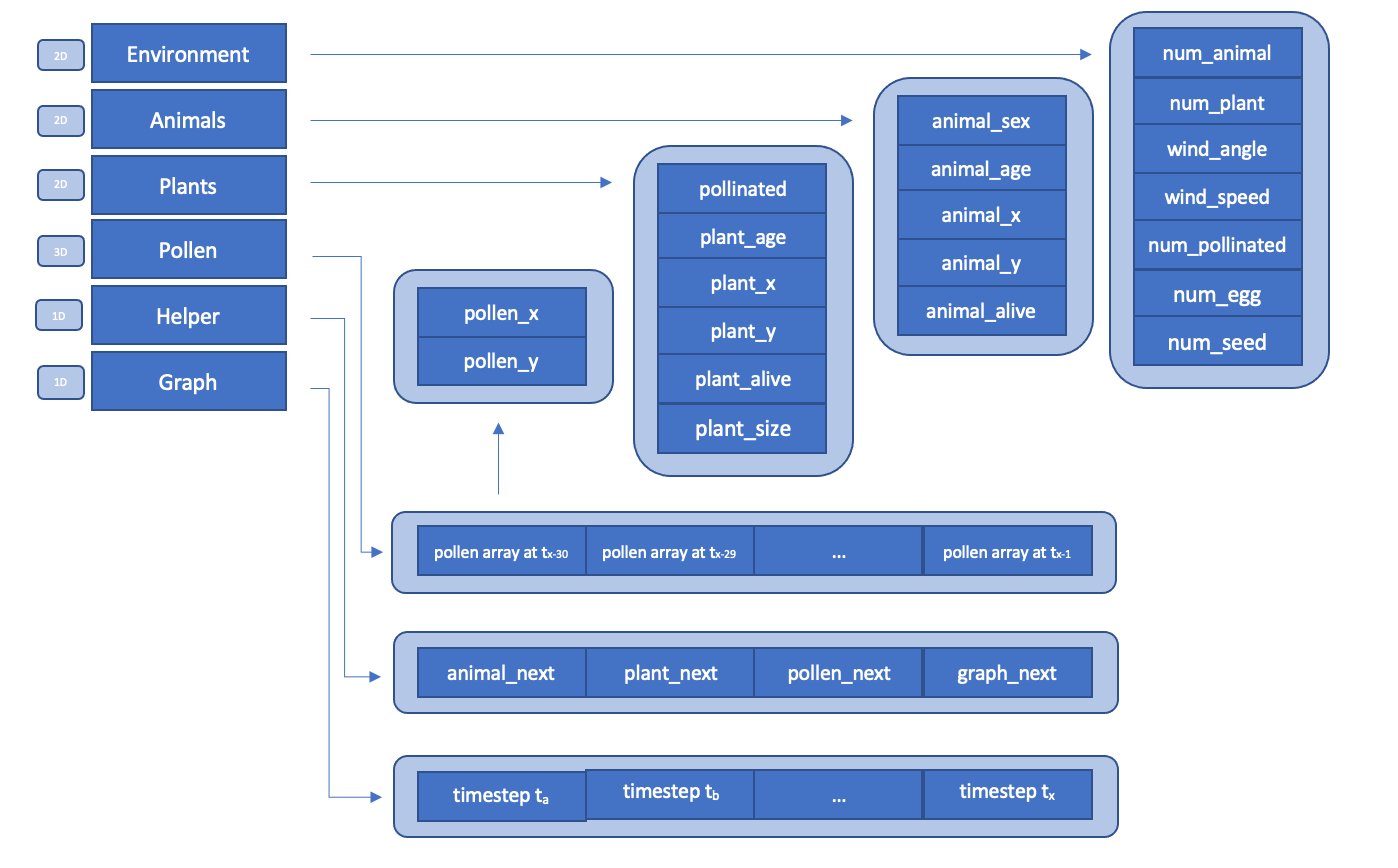
\includegraphics[width=150mm]{figures/array_structure_2.png} 
    \caption{Array Structures of the Model}
    \end{center}
    \end{figure}

In the model, there are box variables (1, 2 and 3D arrays) for Environment, Animals, Plants, Pollen, Helper and Graph. The Environment array has size [total time step, number of environment attributes], where each subarray stores the environment statistics of a day. The Animals array has size [total number of animals in the environment, number of animal attributes], where each subarray stores the attributes of one animal. The Plants array has size [total number of plant clusters in the environment, number of plant attributes], where each subarray stores the attributes of one plant cluster. The Pollen array has size [length of effectiveness, number of pollen grains in each time step, number of pollen attributes], where each subarray stores a list of pollen at a certain date. The Helper array keeps track of the next available space in the Animals, Plants, Pollen and Graph Arrays accordingly. The Graph array is a user-defined list of time steps when the visualization is desired (see Appendix A for a full list of attributes). 

    \begin{table}[!htb]
    \begin{center}
    \begin{tabular}{ l l l}
    Box Variable & Dimension & Size \\
    $Environment$ & 2D & [total time step, number of environment attributes] \\
    $Animals$ & 2D & [number of animals, number of animal attributes] \\
    $Plants$ & 2D & [number of plants, number of plant attributes] \\ 
    $Pollen$ & 3D & [number of effective dates, number of pollen, \\
    && number of pollen attributes]\\
    $Graph$ & 1D & length of user-desired number of dates \\
    $Helper$ & 1D & length of 5 \\
    \end{tabular}
    \caption{\label{tab:table-name}List of Box Variables and properties}
    \end{center}
    \end{table}
\pagebreak

\subsubsection{Simulation Implementation} 

\noindent \textbf{Time step:} the simulation time step in the simulation is 1, which means that all existing probabilities are daily. Therefore, it is currently not possible to make adjustment to time step. \\

\noindent \textbf{Initialization:} Locations of plant clusters and pollinators are, and the initial age of all plants and pollinators are zero. \\

\noindent \textbf{Main simulation:}\\
    \indent loop through the total number time steps with increment of one day \\
    \indent \indent update environment conditions \\
    \indent \indent update pollen array indexes \\
    \indent \indent loop through each plant \\
    \indent \indent \indent update plant age \\
    \indent \indent \indent condition 1: plant is still an alive seed \\
    \indent \indent \indent \indent check survival probability, related to absolute temperature difference\\
    \indent \indent \indent condition 2: plant just becomes an alive plant \\
    \indent \indent \indent \indent update number of alive plants and seeds \\
    \indent \indent \indent condition 3: plant is an alive plant before maturity \\
    \indent \indent \indent \indent may produce pollen \\
    \indent \indent \indent condition 4: plant is an alive plant during seed producing \\
    \indent \indent \indent \indent may produce seeds \\
    \indent \indent \indent condition 5: plant is about to die \\
    \indent \indent \indent \indent update number of alive plants \\
    \indent \indent end plant loop \\
    \indent \indent if with enough pollen \\
    \indent \indent \indent merge pollen arrays to obtain attractive pollen list \\
    \indent \indent \indent find the locations of high pollen densities \\
    \indent \indent end if\\
    \indent \indent loop through each animal \\
    \indent \indent \indent update animal age \\
    \indent \indent \indent condition 1: animal is still an alive egg \\
    \indent \indent \indent \indent check survival probability, related to absolute temperature difference \\
    \indent \indent \indent condition 2: animal just becomes an alive animal \\
    \indent \indent \indent \indent update number of alive animals and eggs \\
    \indent \indent \indent condition 3: animal is female \\
    \indent \indent \indent \indent may produce eggs \\
    \indent \indent \indent condition 4: animal is an alive animal \\
    \indent \indent \indent \indent sub-condition 1: not enough pollen\\
    \indent \indent \indent \indent \indent movement based on wind\\
    \indent \indent \indent \indent sub-condition 2: enough pollen\\
    \indent \indent \indent \indent loop through plants \\
    \indent \indent \indent \indent \indent pollinate plants if nearby and within visiting capacity \\
    \indent \indent \indent \indent \indent movement based on pollen densities with wind disturbance probability\\
    \indent \indent \indent condition 5: animal is about to die \\
    \indent \indent \indent \indent update number of alive animals \\
    \indent \indent end animal loop \\
    
\noindent \textbf{Visualization:}\\ 
    \indent Animal and Plant Populations vs. Time\\
    \indent Egg and Seed Production vs. Time\\
    \indent Spatial Locations of Alive/Dead Plant and Animal Species Individuals\\
    \indent Spatial Locations of Attractive Pollen\\\

\subsection{Validation}
The validation of the model should be considered at two scales: the populations and communities scale and then individual plant cluster or pollinator scale. It is important for both the community dynamics and the individual behaviors to match the expected results. The presented validation test is a simulation over a two year period with time step 1 day. The environment is initialized with a landscape size of $160\times160$, 20 animals and 100 plant clusters in the environment. The maximum wind speed in the environment is 5, and the pollinators will $100\%$ pollinate the plant cluster successfully assuming no wind in the environment. The temperature of the environment would stay constant within the simulation time frame. All plant clusters and animals are initialized with age of 1 at the beginning of the simulation. The female animals would lay 10 eggs each time, and the survival probability of eggs is $80\%$ each day. After 10 days, the eggs will become alive animals that can move freely in the environment. All animals die at age 365. The plant species can be pollinated before age 180 days, approximately half of their life span. During a following period of 120 days the plant clusters are allowed to produce seeds, dispersed through wind and with different sizes. After landing successfully, it takes 60 days for the seed to become an alive plant cluster.

\subsubsection{Match of Inter-species Agent Behaviors}

    \begin{figure}[!htb]
    \begin{center}
    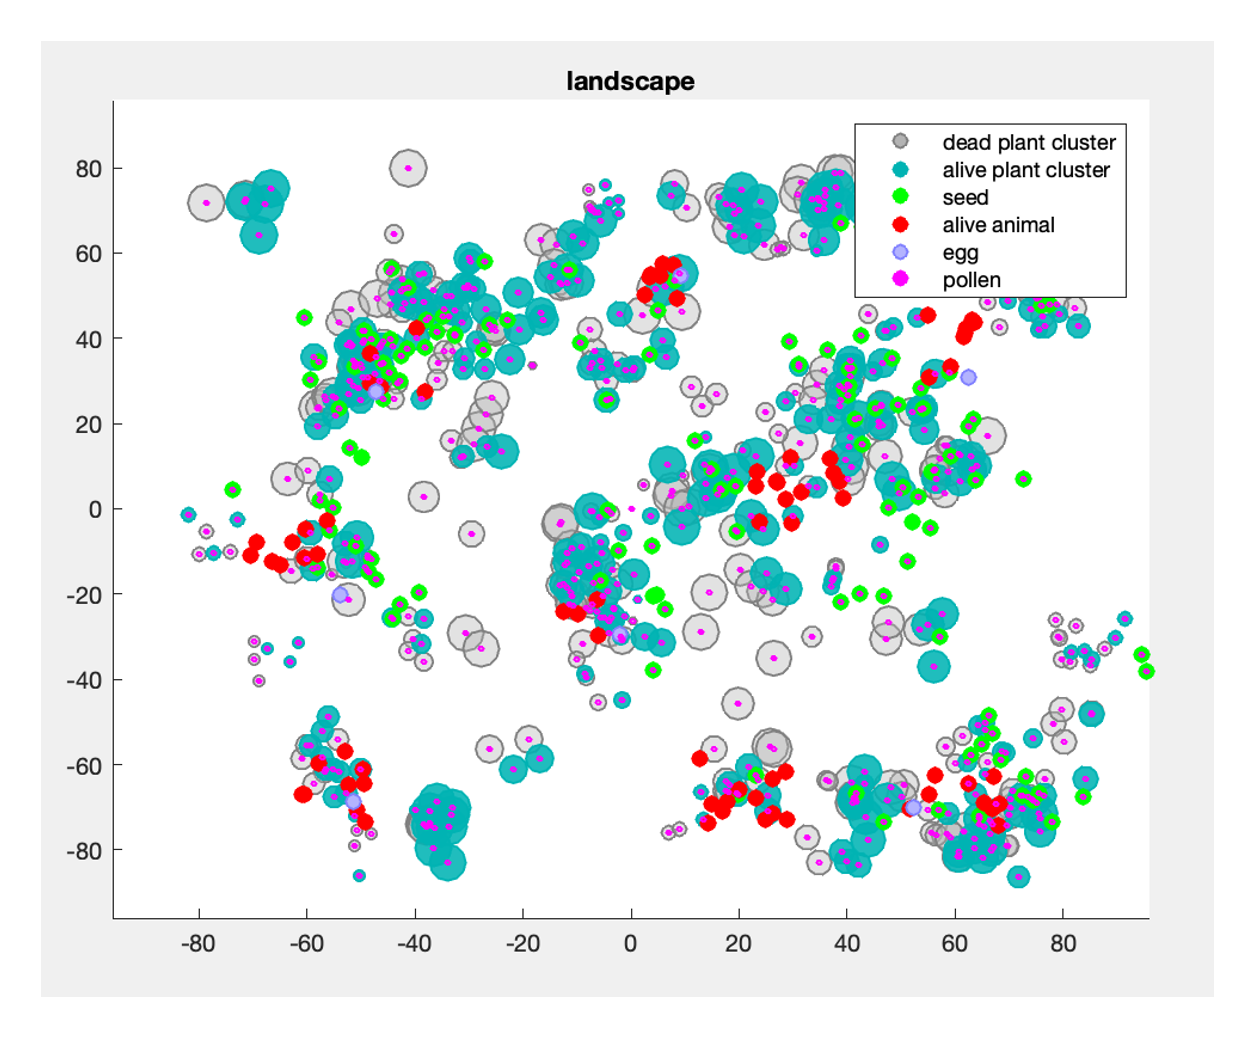
\includegraphics[width=100mm]{figures/validation_4.png} 
    \caption{Example Population Distribution and Pollen Distribution over 2 years}
    \end{center}
    \end{figure}

The above figure shows that the animals tend to move to areas with high pollen densities, with a few pollinators spreading over the rest of the plant clusters. The plant clusters follow a seed, growth, mature, dead life cycle, and the animals would be in either egg stage with fixed locations or individual agents that are attracted by produced pollen. A potential risk is that it is possible for the pollinators to visit areas with relatively high pollen density but relatively low alive plant density, which will result in animal reproduction due to the reward of pollen as food but failure in pollination services since there could be no alive plants nearby. Pollen grains are plotted along with plant and pollinator species to show the visual match between pollinator distribution and pollen distribution. 

Particularly in this simulation, the wind effect on pollen is removed and the disturbance effect on animals foraging behaviors are removed. The animals are expected to visit areas with high plant cluster densities. Note that they would visit areas with high plant cluster densities rather than high plant densities because the probability of producing pollen is imposed on each plant cluster rather than each plant. See Appendix C for default simulation parameters. 
    
\subsubsection{Model Evaluation} 
In a two-species pollination-based mutualism environment, the model needs to be tested against the field data with statistical results indicating the level of significance between sample data and model data.

\section{Simulations and Results}
\subsection{Effects of species-specific traits}
(i) the effects of plant traits and spatial distribution, including plant density, species spatial pattern and relative attractiveness due to pollination services

\subsubsection{Simulation Experiment 1: initial plant density vs. ending plant density}

    \begin{figure}[!htb]
    \begin{center}
    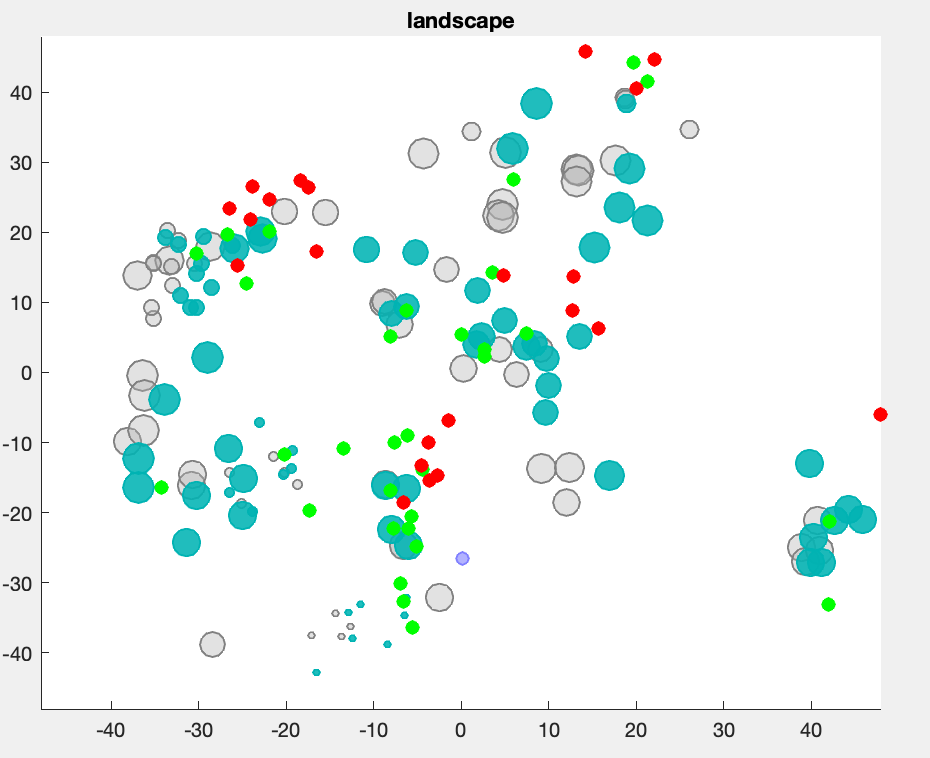
\includegraphics[width=50mm]{figures/s1_1.png} 
    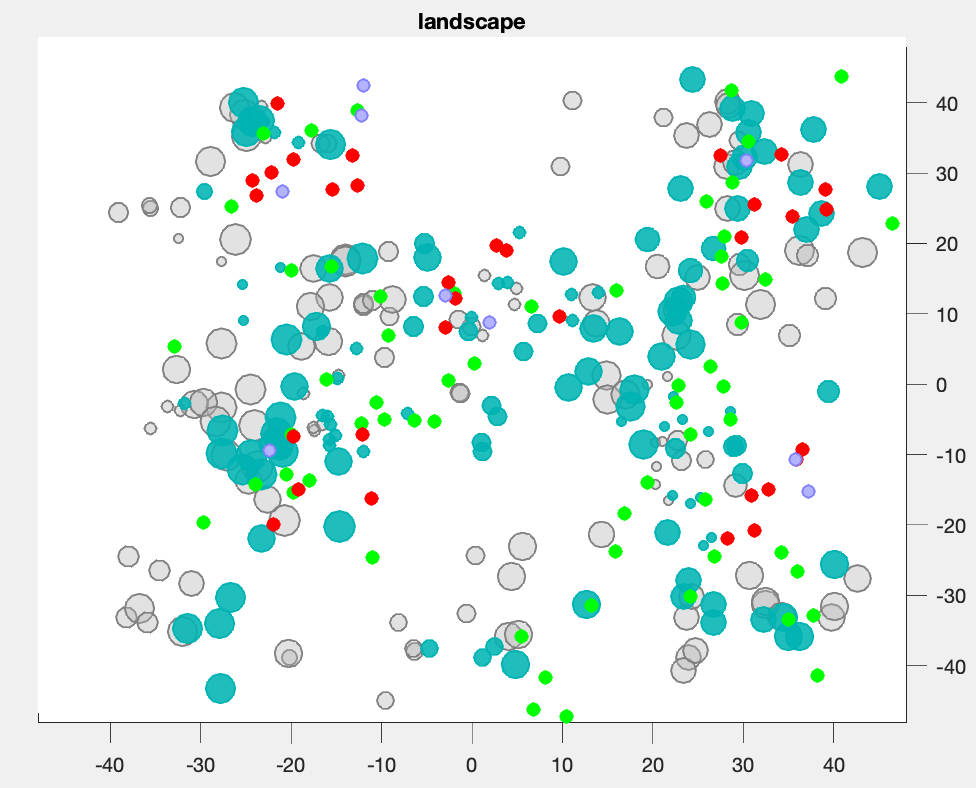
\includegraphics[width=50mm]{figures/s1_2.png} 
    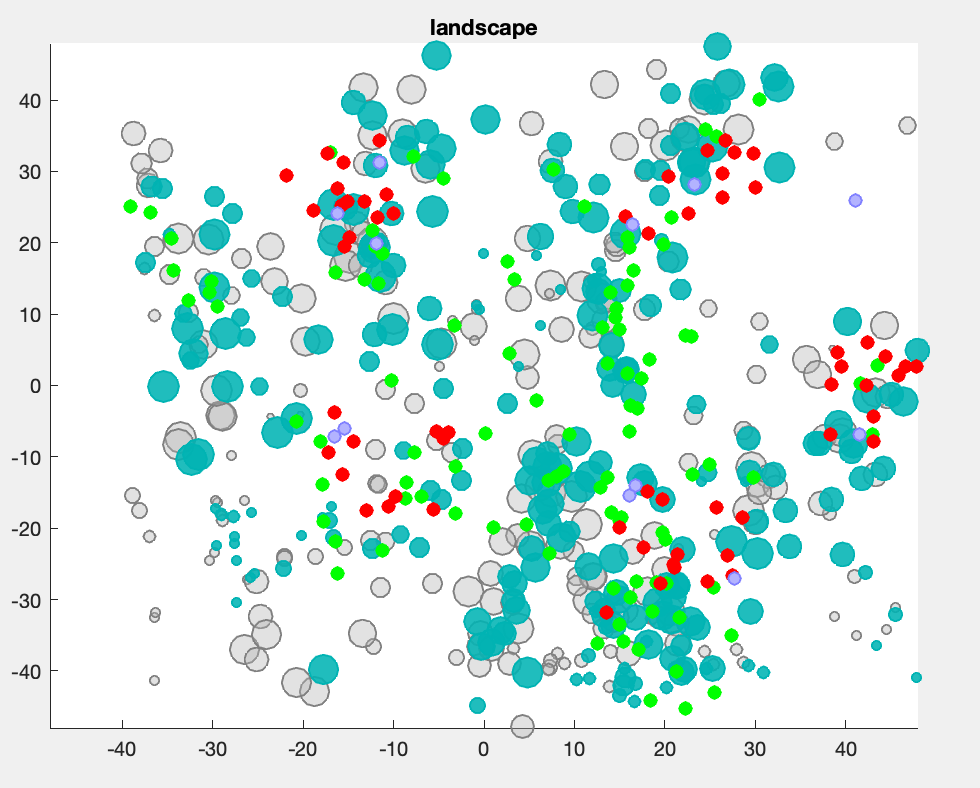
\includegraphics[width=50mm]{figures/s1_3.png} 
    \caption{Distributions with initial density = 0.5, 1 and 2 (default simulation)}
    \end{center}
    \end{figure}
    
The modified parameter in the simulation experiment is the number of initial plant clusters. Initial plant density is evaluated using 
        \begin{center}
        $initial$ $density$ = $num\_plant$ $\div$ $init\_size$
        \end{center}
Note that the plant density here is essentially plant cluster density rather than individual plant density. From the simulation results, when initial density is around 1, the spatial plant density is the smallest over time: the individual plant clusters would be able to move from the initial plant clusters compared to smaller and larger initial density. When the initial density is small, the plant clusters are too dispersed and they will gradually form clustered plant clusters in time. When the initial density is large, the plant clusters also would not move away because the pollinators only visit dense plant clusters, making the clustered plant clusters more dense. 

However, it is also reasonable to modified the initial plant cluster size in the environment. In this case, initial plant density is evaluated using 
        \begin{center}
        $initial$ $density$ = $init\_cluster\_size$ $\div$ $init\_size$
        \end{center}
After simulations with 0.1, 0.5, 1 initial densities, the results do not show a notable change in plant cluster distribution. 
    
\subsubsection{Simulation Experiment 2: effect of plant life cycle and population statistics}
    \begin{figure}[!htb]
    \begin{center}
    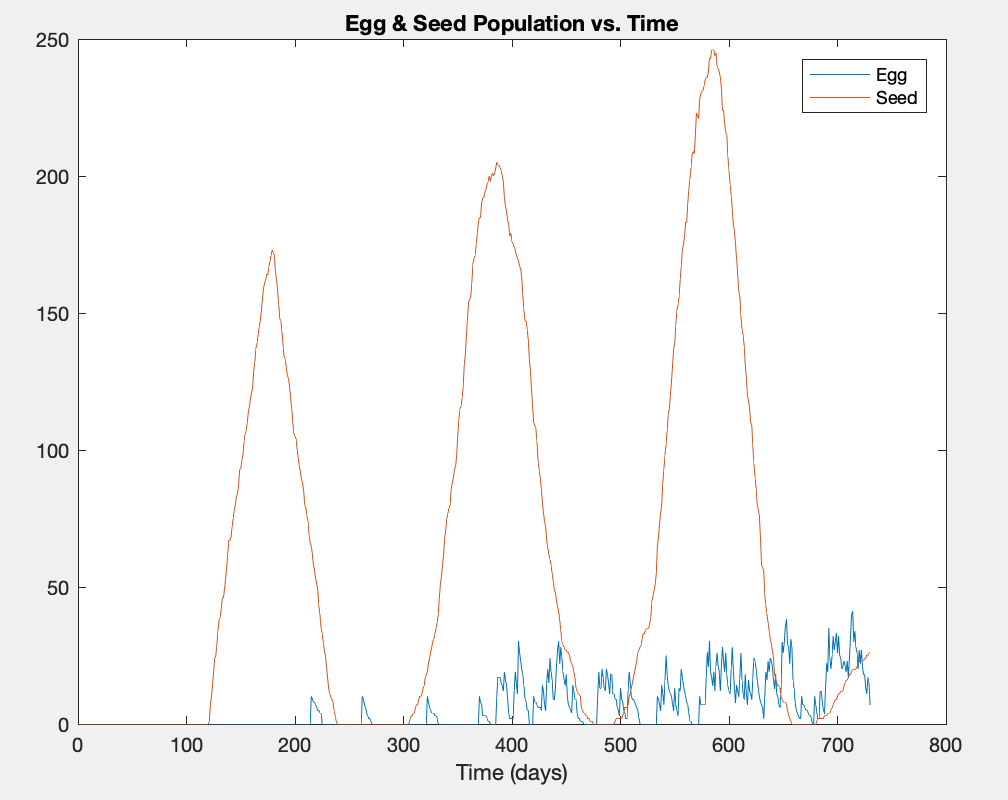
\includegraphics[width=53mm]{figures/s2_3.png} 
    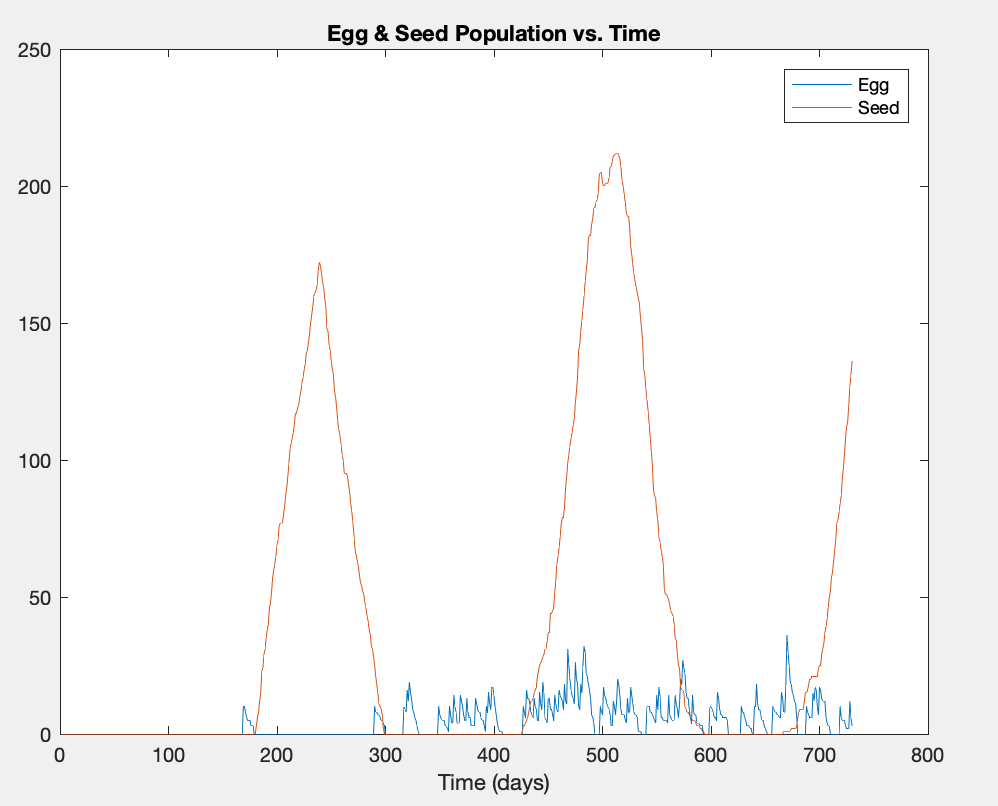
\includegraphics[width=52mm]{figures/s2_1.png} 
    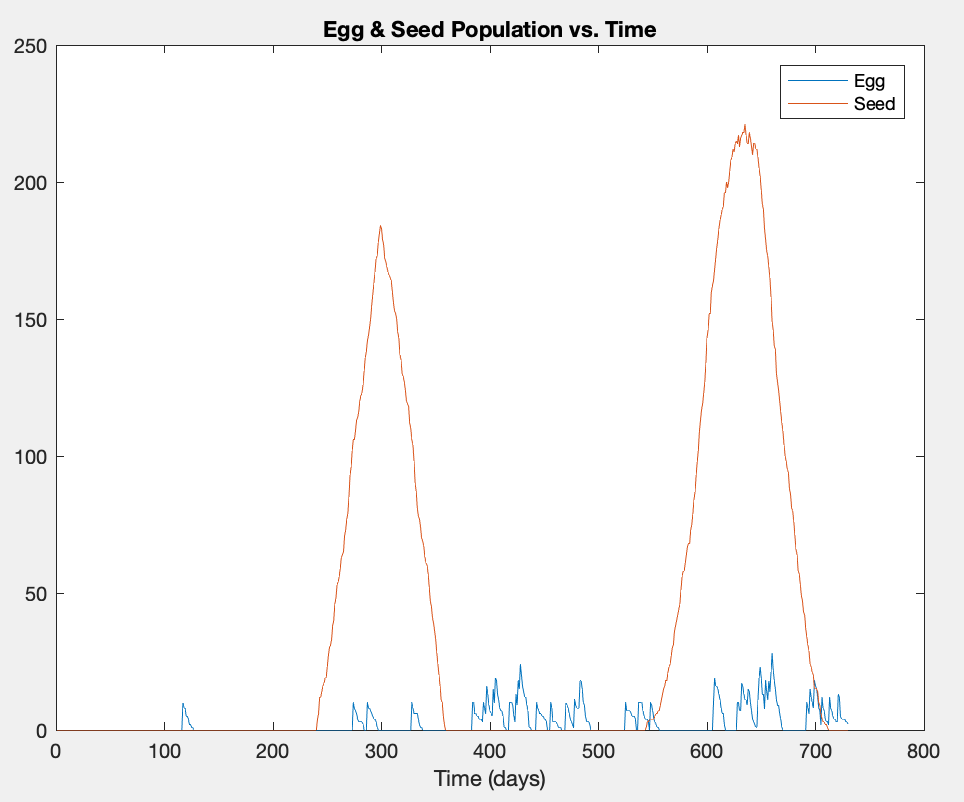
\includegraphics[width=50mm]{figures/s2_2.png} 
    \caption{Distributions with $maturity\_date$ = 120, 180 and 240 (default simulation)}
    \end{center}
    \end{figure}
    
The modified parameter in the simulation experiment is the number of dates before maturity, which is also the number of dates the plants can be pollinated. The simulation results show that increasing plant maturity dates would result in longer cycles of seed productions and decreasing number of seed production. This will also decrease the frequency and number of egg production because more plants clusters would lead to decreasing pollen production. 

    \begin{figure}[!htb]
    \begin{center}
    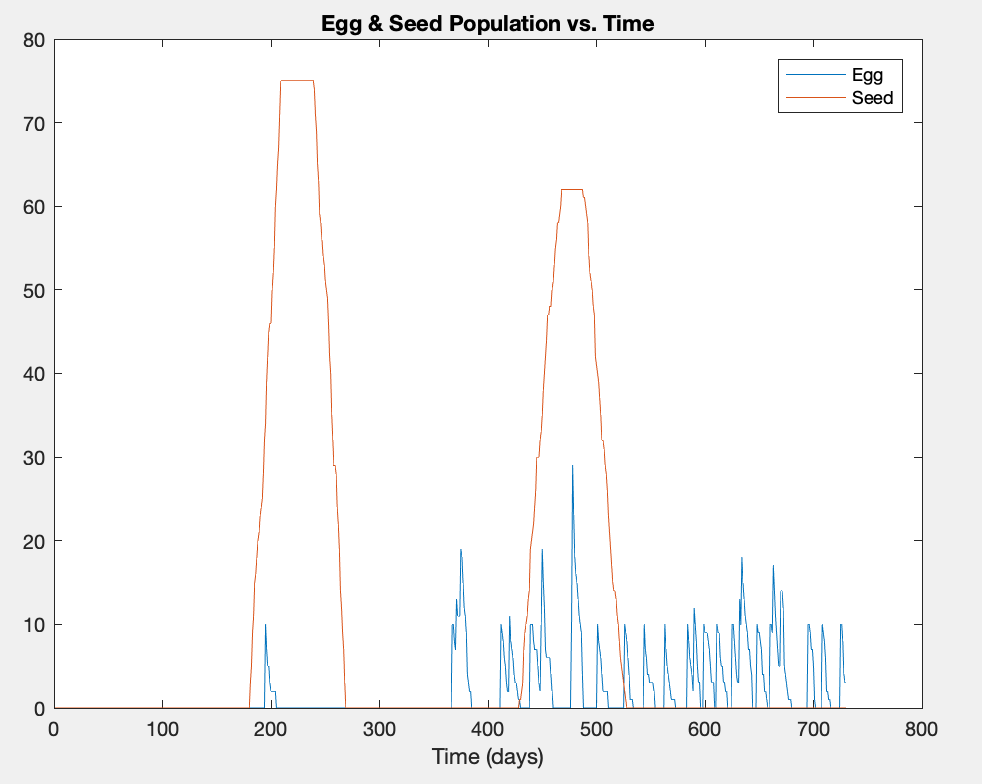
\includegraphics[width=52mm]{figures/s2_4.png} 
    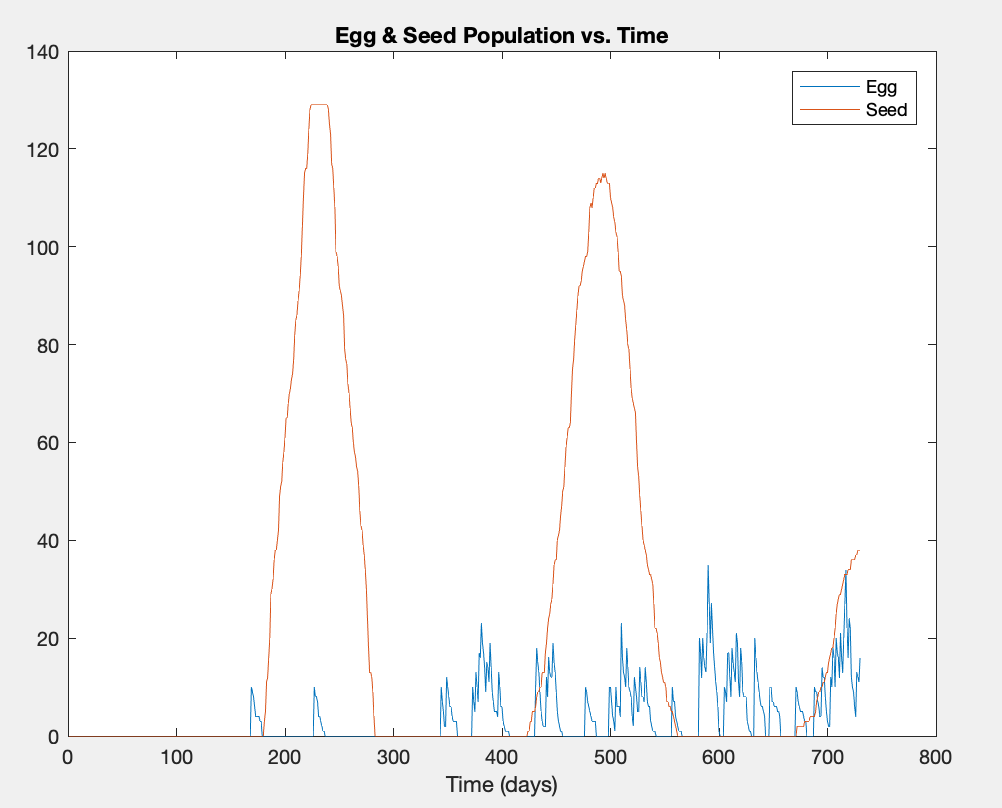
\includegraphics[width=50mm]{figures/s2_5.png} 
    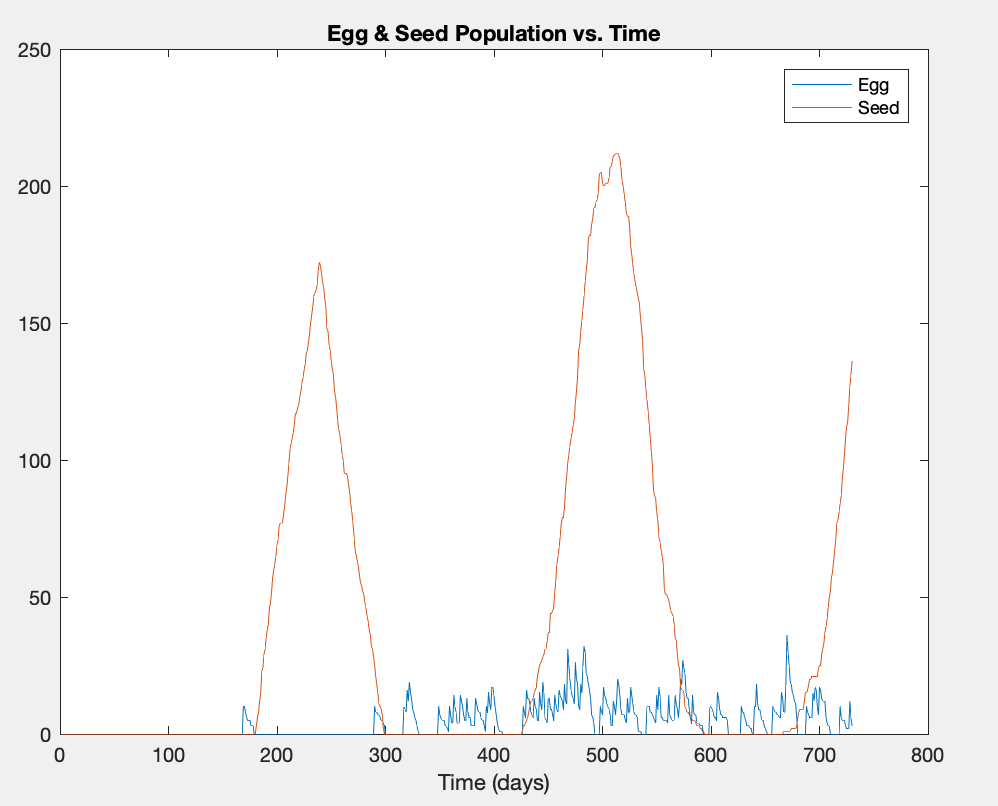
\includegraphics[width=50mm]{figures/s2_1.png} 
    \caption{Distributions with $seed\_period$ = 30, 45 and 60 (default simulation)}
    \end{center}
    \end{figure}
Note that the figures are different in scales. The modified parameter in the simulation experiment is the number of dates that the plant species is able to produce and disperse seeds. The simulation results show that increasing seed producing period would result in shorter cycles of seed productions and increasing number of seed production. This, however, does not seem to lead to changes in the frequency and number of egg production as from the figure no noticeable difference in number and frequency of eggs produced (using the same scale).

    \begin{figure}[!htb]
    \begin{center}
    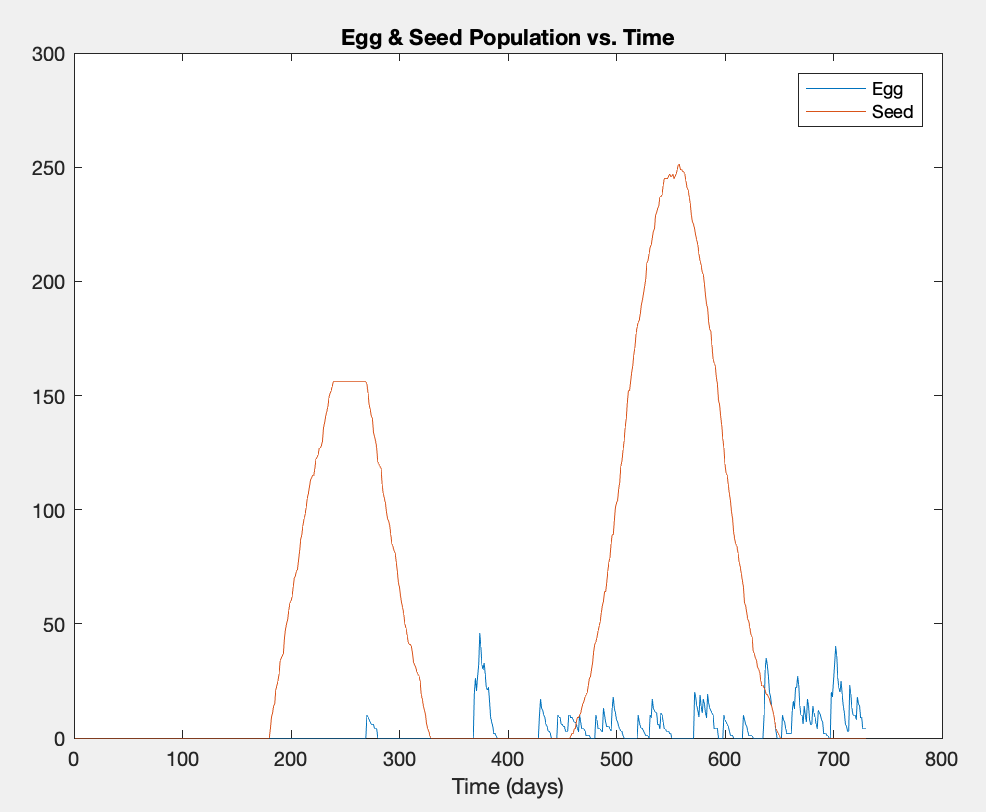
\includegraphics[width=50mm]{figures/s2_6.png} 
    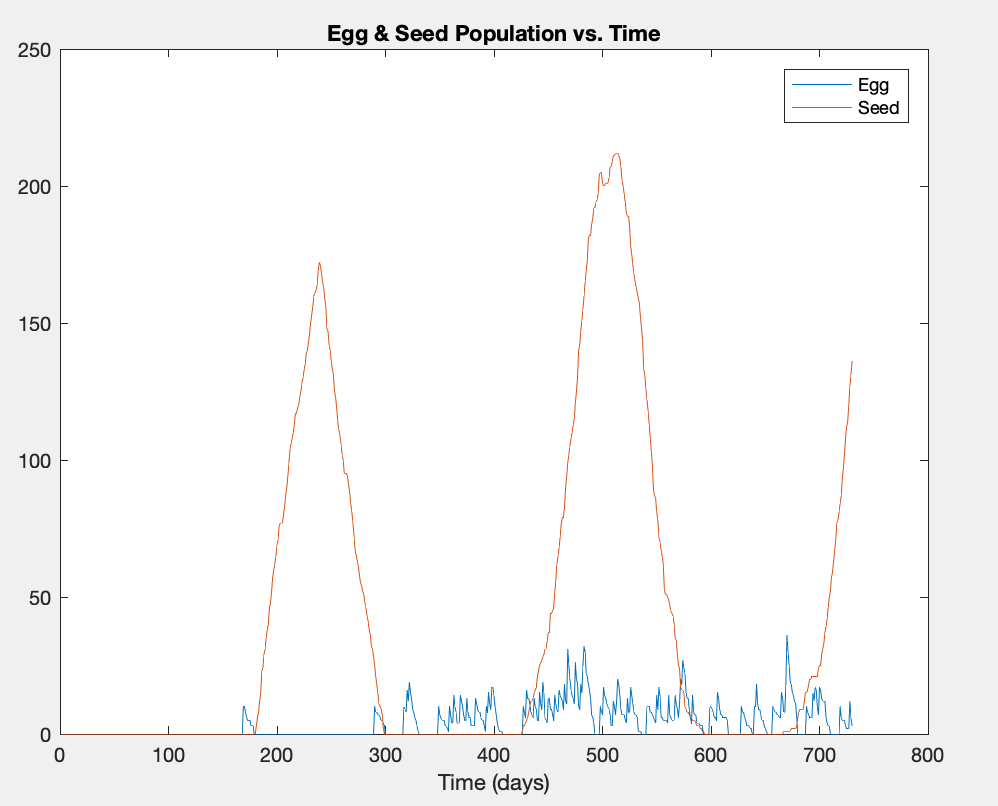
\includegraphics[width=50mm]{figures/s2_1.png} 
    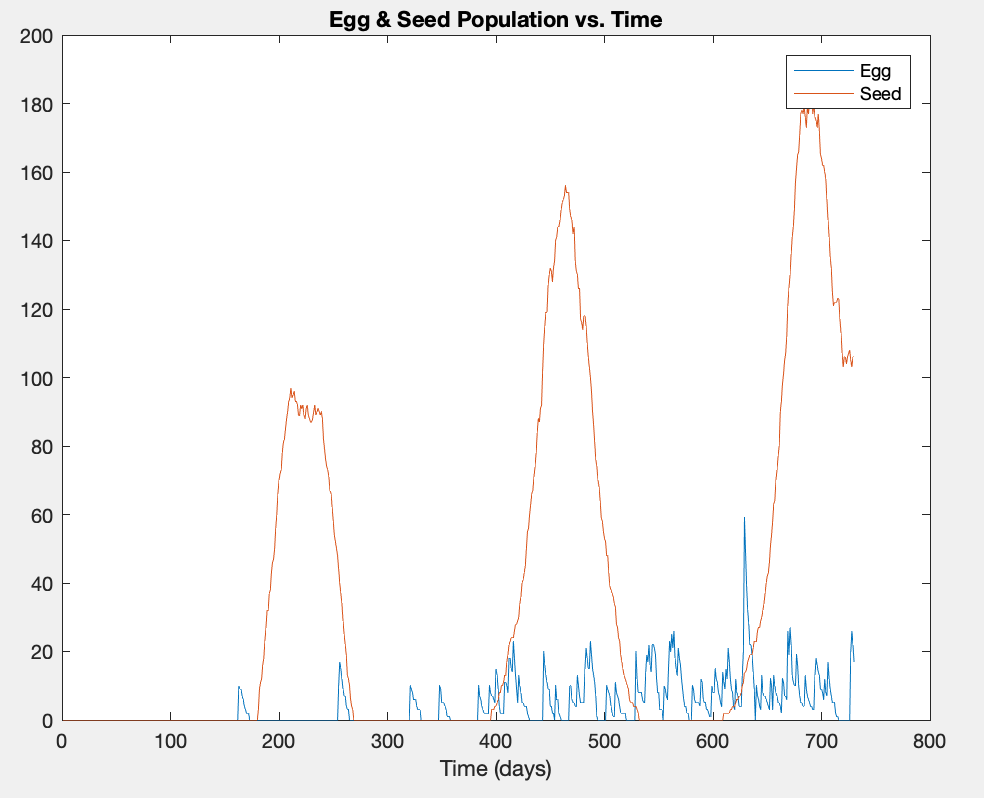
\includegraphics[width=50mm]{figures/s2_7.png} 
    \caption{Distributions with $seed\_stage$ = 30, 60 and 90 (default simulation)}
    \end{center}
    \end{figure}

Note that the figures are different in scales. The modified parameter in the simulation experiment is the number of dates that the seed becomes a plant. The simulation results show that increasing number of seed period would result in shorter cycles of seed productions but decreasing number of seed production. This, however, does not seem to lead to changes in the frequency and number of egg production as from the figure no noticeable difference in number and frequency of eggs produced (using the same scale).
    
\subsection{Effects of plant-animal interaction}
(ii) the effects of pollinator behaviors on the plant species across generations

\subsubsection{Simulation Experiment 3: effect of pollinator visiting behaviors on environment dynamics}

    \begin{figure}[!htb]
    \begin{center}
    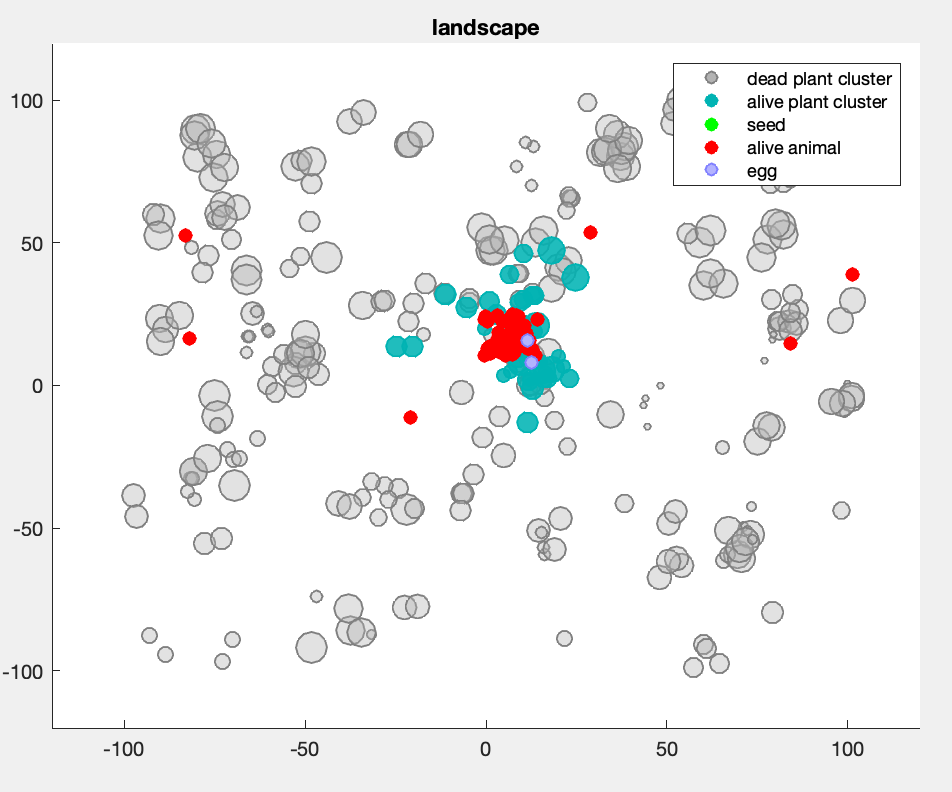
\includegraphics[width=78mm]{figures/s3_1.png} 
    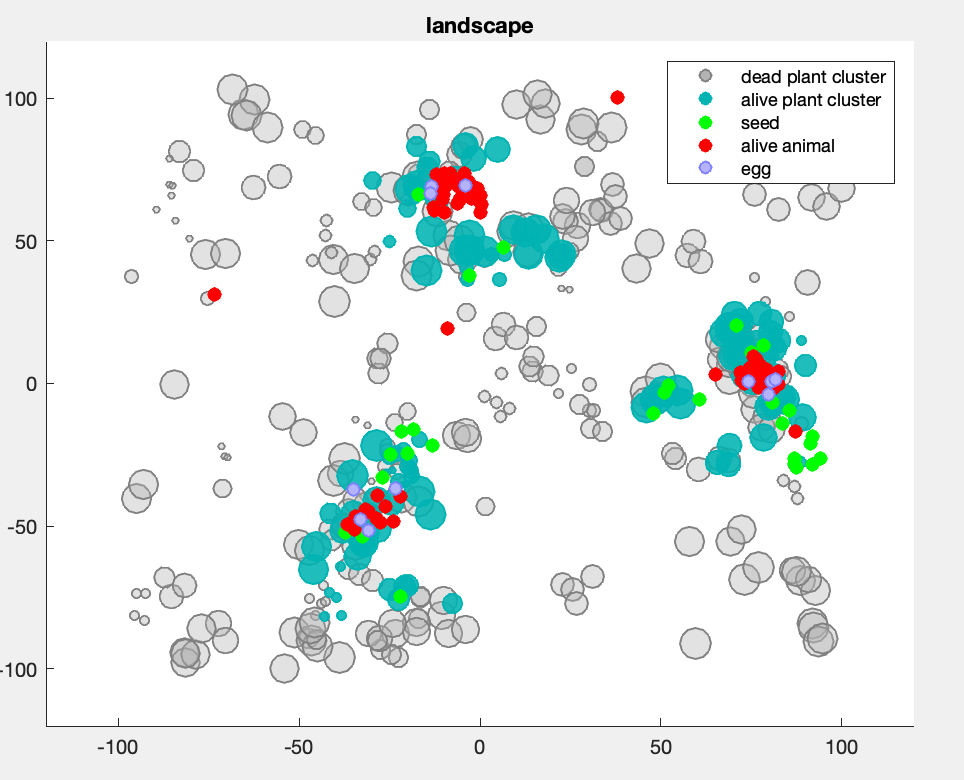
\includegraphics[width=80mm]{figures/s3_2.png} 
    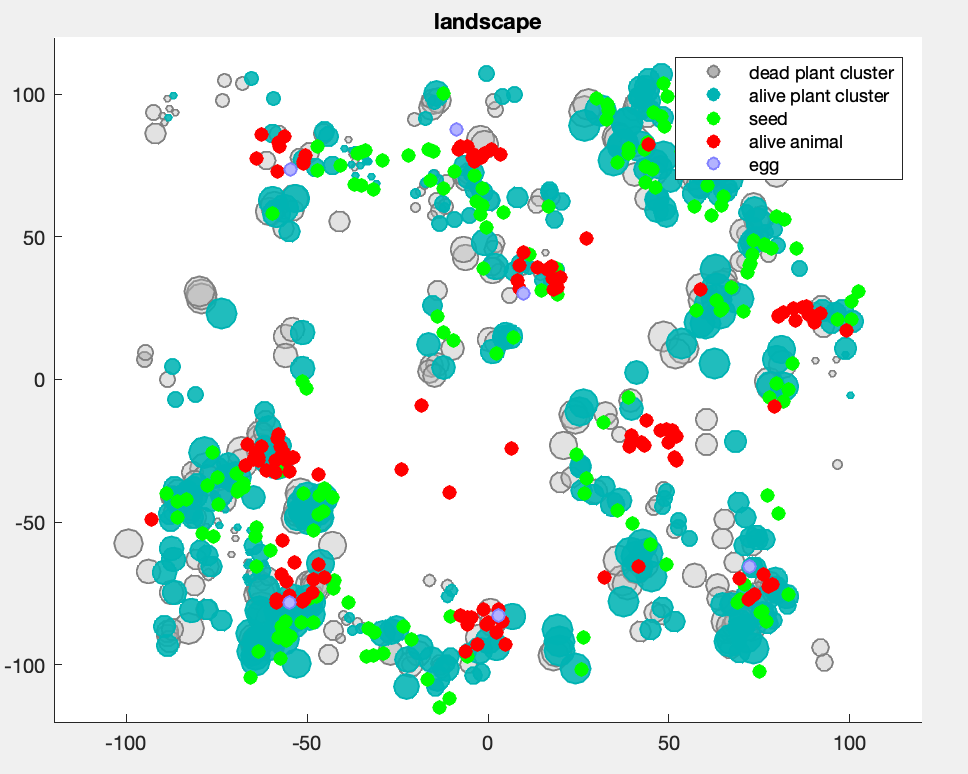
\includegraphics[width=78mm]{figures/s3_3.png}
    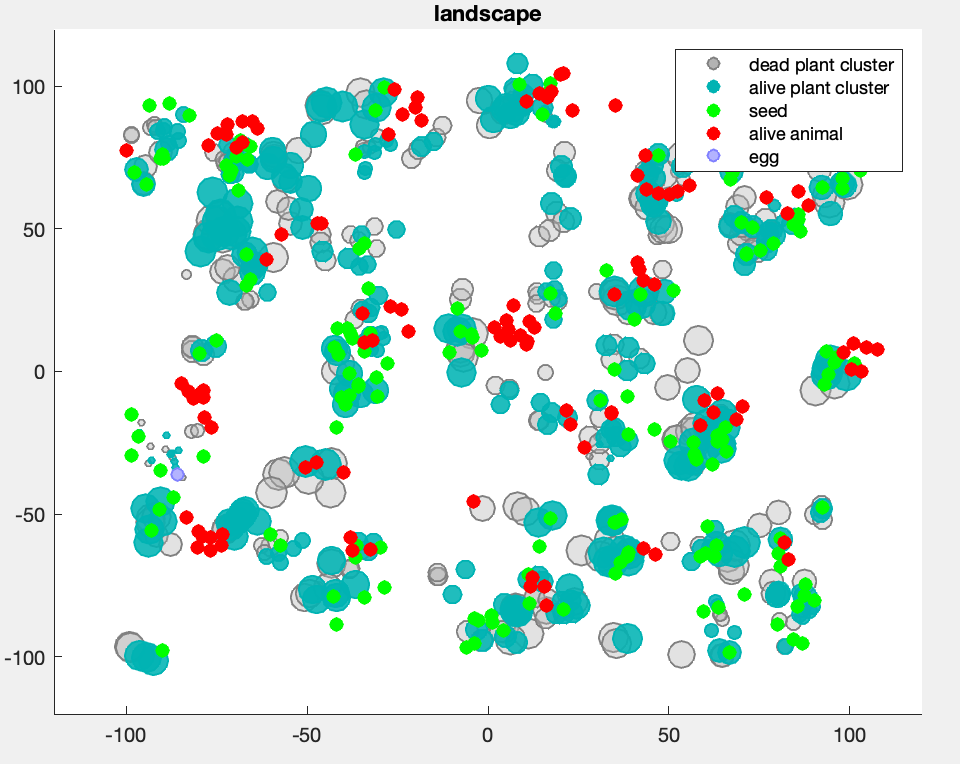
\includegraphics[width=80mm]{figures/s3_4.png}
    \caption{Distributions with $init\_size$ = 100 (default simulation) and n = 1, 3, 10, 20}
    \end{center}
    \end{figure}

The experiment hypothesis is that though there is an area in the environment with “the highest density,” pollinators would not all visit the that particular area and would spread out to multiple locations instead. Note that the assumption in the model is that the animals would not be attracted to one particular plant cluster, but rather an area with high pollen density. 

Simulation results indicate that it is very unlikely for the pollinators to visit one particular area with the highest pollen density and ignore relatively low pollen density areas. This could be due to pollinators failing to recognize the place with the highest plant density, or that the pollinators would not compete for food and would rather visit another cluster with less pollen grains. Simulation results are not able to make any conclusion regarding why or why not the pollinators will not all visit the area with the highest pollen density, but the result shows that if pollen density is the absolute prioritized standard with no exception, the plant species may quickly go extinct as the plant population would experience quick and huge deduction, with a small number of plants survived. Since the plants can only produce limited pollen grains, the animal reproduction rate would significantly low and therefore may also result in extinction of the pollinator species.

\subsection{Effects of environmental disturbance}
(iii) how the plant-plant interactions impact and are impacted the environmental system considering factors like wind and temperature

\subsubsection{Simulation Experiment 4: effect of wind on and species reproduction}
The table below shows the effects of maximum wind speed has on species reproduction.
    \begin{table}[!htb]
    \begin{center}
    \begin{tabular}{ c c c }
    Maximum Wind Speed & Average Number of Eggs & Average Number of Seed \\
    1 & 4.293 & 42.889 \\
    2 & 4.133 & 42.006 \\
    5 & 4.332 & 40.874 \\ 
    8 & 3.994 & 42.063 \\
    10 & 4.267 & 41.782 \\
    \end{tabular}
    \caption{\label{tab:table-name} Averaged 10-time simulation results from initial landscape 80*80 (default simulation)}
    \end{center}
    \end{table}

The modified parameter in the simulation experiment is maximum wind speed. The average number of eggs is the averaged egg production amount across all time steps, and the average number of seed is the averaged seed production amount across all time steps. There does not seems to be a significant difference or pattern across different maximum wind speed. The presented results are the averaged results running 10 simulations using identical parameter values.

\subsubsection{Simulation Experiment 5: effect of wind on plant locations across generations}
The table below shows the effects of maximum wind speed has on the distribution of plant cluster locations. The exceeding distance is obtained using
    \begin{center}
    $exceeding$ $distance$ = Euclidean distance between plant and origin - $init\_size$
    \end{center}

    \begin{table}[!htb]
    \begin{center}
    \begin{tabular}{ c c c }
    Maximum Wind Speed & Maximum Exceeding Distance & Average Exceeding Distance \\
    1 & 2.52 & 0.97 \\
    2 & 3.08 & 2.24 \\
    5 & 8.92 & 4.80 \\ 
    8 & 14.71 & 4.92 \\
    10 & 16.02 & 5.44\\
    \end{tabular}
    \caption{\label{tab:table-name} Averaged 10-time simulation results from initial landscape 80*80 (default simulation)}
    \end{center}
    \end{table}

The modified parameter in the simulation experiment is maximum wind speed. The maximum exceeding distance is obtained looping through all plant clusters, both alive and dead, and finding the maximum plant cluster location that move the furthest from the initial landscape location. The average exceeding distance is the averaged exceeding distance from the initial landscape of all plant clusters located outside the initial landscape. Simulation results show that increasing wind speed would result in increasing movement of plant species, evaluated by exceeding distance described above. The presented results are the averaged results running 10 simulations using identical parameter values.

\section{Discussion}
\subsection{Discussion on example hypothesis testing results}

The initial plant numbers with respect to wind would have effects on plant cluster densities and clustering behaviors. A particular low or high initial densities would result either in individual plant clusters forming clusters or clustered plant clusters becoming more condensed. 

Changes in length of the three stages of a plant's life cycles would have conflicting effects on seed and egg production. The table below shows a summary of the effect:
    \begin{table}[!htb]
    \begin{center}
    \begin{tabular}{ l c c c c }
    Parameter & Seed Production Cycle & Seed Production Amount \\
    $maturity\_date$ & Increase & Decrease\\
    $seed\_period$ & Decrease & Increase\\
    $seed\_stage$ & Decrease & Decrease\\
    &&\\
    Parameter & Egg Production Frequency & Egg Production Amount \\
    $maturity\_date$ & Decrease & Decrease \\
    $seed\_period$ & No Effect & No Effect \\
    $seed\_stage$ & No Effect & No Effect \\
    \end{tabular}
    \caption{\label{tab:table-name} Effect of changes in different stages of plant life cycle on species reproduction}
    \end{center}
    \end{table}

Additionally, simulation results indicate that it is very unlikely for the pollinators to visit one particular area with the highest pollen density and ignore relatively low pollen density areas. A reasonable default foraging behaviors may be considered as 
        \begin{center}
        $n$ = $init\_size$ $\div$ 10 + 1
        \end{center}
after running multiple simulations with different $init\_size$ and number of spreading groups. Note that if the number of spreading group is equal to the number of alive animals, each animal would go to different block with uniform area of each block. 

With the impact of wind, the plant clusters are able to move outside the initial landscape considering the generational movement of plant clusters. When seed dispersal is dependent on wind, the system with higher wind speed would result in more spatially spreading seed distributions and therefore further movements across three plant generations. However, wind does not seem to have an impact on species reproduction. 

\subsection{Usefulness of the Model}
From the examples presented in this project, the agent-based, spatially explicit model can bring significant benefits in investigating two-species pollination based mutualism. The usefulness of the model can be evaluated considering the user-defined parameters incorporated in the model. Researchers may use the model simulating a two-species pollinated-based mutualism system when:
\begin{itemize}
  \item spatial patterns are involved and the agents' positions are not fixed
  \item scales of environment and species densities are involved
  \item species life cycles are involved and reproduction of species are dependent (pollination for plants and food for pollinators)
  \item environmental factors including wind motion and temperature are involved
\end{itemize}

\section{Conclusion}
This spatially explicit and agent-based model can be used to represent complex spatial and behavioral interactions among different pollinator and plant species and help investigate effects of plant traits, pollinator behavior, and spatial locations in a two-species shared pollination service system. The model can be used to evaluate relative effects of shared pollination services with respect to species-specific and environment-species traits and may further incorporate additional plant and pollinator traits. Future research may focus on incorporating new features into the model, including flower color, plant hormones, and different foraging behaviors. In addition, researcher may also use the model to generate causal conclusions between two-species pollination-based interaction through factor-controlled analysis and subsequently contribute to nature conservation of both the plant and the pollinator species.
\pagebreak 

\section{References}
\bibliography{citation}
\bibliographystyle{elsarticle-num}
\pagebreak

\appendix 
\section{Full List of Variables}

\subsection{\textbf{Environment, Animals, Plants Attributes}}
\begin{table}[!htb]
\begin{tabular}{ l l }
 $num\_animal$ & the number of alive animals in the environment \\
 $num\_plant$ & the number of alive plants in the environment \\
 $wind\_angle$ & wind direction is defined as the direction the wind is coming from \\ 
 $wind\_speed$ & wind speed is defined as the scalar quantity of the wind, \\
 & a randomized magnitude between 0 and maximum wind speed \\
 $num\_egg$ & the number of eggs in the environment \\
 $num\_seed$ & the number of seeds in the environment \\
 $temp$ & the temperature in Celsius degree in the environment \\
\end{tabular}
\caption{\label{tab:table-name}List of Environment Attributes}
\end{table}

\begin{table}[!htb]
\begin{tabular}{ l l }
 $animal\_sex$ & 0 represents male and 1 represents female\\
 $animal\_age$ & integer, age of the animal \\ 
 $animal\_x$ & double, x position of the animal \\
 $animal\_y$ & double, y position of the animal \\
 $animal\_alive$ & integer, whether the animal is alive or not\\
\end{tabular}
\caption{\label{tab:table-name}List of Animal Attributes}
\end{table}

\begin{table}[!htb]
\begin{tabular}{ l l }
 $pollinated$ & whether the plant cluster is pollinated (1) or not (0)\\
 $plant\_age$ & integer, age of the plant cluster \\ 
 $plant\_x$ & double, x position of the plant cluster \\
 $plant\_y$ & double, y position of the plant cluster \\
 $plant\_alive$ & integer, whether the plant cluster is alive or not\\
 $plant\_size$ & integer, size of the plant cluster\\
\end{tabular}
\caption{\label{tab:table-name}List of Plant Cluster Attributes}
\end{table}

\begin{table}[!htb]
\begin{tabular}{ l l }
 $pollen\_x$ & double, x position of the pollen \\
 $pollen\_y$ & double, y position of the pollen \\
\end{tabular}
\caption{\label{tab:table-name}List of Pollen Attributes}
\end{table}

\pagebreak
\subsection{\textbf{Environment, Animals, Plants Constants (User-defined)}}
\begin{table}[!htb]
\begin{tabular}{ l l }
 $max\_wind\_speed$ & the maximum wind speed allowed in the environment \\
 $max\_pollination\_success\_rate$ & pollination success rate when there is no wind \\
 $prob\_disturb$ & the probability of wind disturbance on animal \\
 & foraging behaviors \\
\end{tabular}
\caption{\label{tab:table-name}List of Environment-related Constants}
\end{table}

\begin{table}[!htb]
\begin{tabular}{ l l }
 $egg\_stage$ & number of days before the egg becomes an animal \\ 
 $num\_egg$ & number of eggs a female animal lays \\ 
 $prob\_egg\_survival$ & survival probability of each egg per day \\
 $best\_temp\_egg$ & the most comfortable temperature for egg survival \\
 $visit\_capacity$ & the maximum number of visits per day of each animal \\
\end{tabular}
\caption{\label{tab:table-name}List of Animal-related Constants}
\end{table}

\begin{table}[!htb]
\begin{tabular}{ l l }
 $seed\_stage$ & number of days before the seed becomes a plant \\ 
 $plant\_maturity\_date$ & number of seedling days, when the plant can be pollinated \\
 & but cannot produce seeds\\ 
 $seed\_period$ & number of days the plant species can produce \\
 & and distribute seeds \\ 
 $prob\_landing$ & probability of the seed landing successfully in the environment \\ 
 $prob\_seed\_survival$ & survival probability of each seed per day \\
 $best\_temp\_seed$ & the most comfortable temperature for seed survival \\
 $prob\_pollen$ & 0.95 \\
\end{tabular}
\caption{\label{tab:table-name}List of Plant-related Constants}
\end{table}

\subsection{\textbf{Initial Conditions (User-defined)}}
\begin{table}[!htb]
\begin{tabular}{ l l }
 $init\_size$ & initial size of the landscape\\
 $init\_num\_animal$ & initial number of animals in the environment \\ 
 $init\_num\_plant$ & initial number of plants in the environment \\
 $init\_cluster\_size$ & initial maximum size of the plant clusters \\
 $wind\_list$ & (optional) initialize with a full list of wind motion \\
 $temperature\_list$ & (optional) initialize with a full list of temperatures \\
\end{tabular}
\caption{\label{tab:table-name}Initial Conditions of the Environment}
\end{table}
\pagebreak 


\section{Full List of Validations}
\subsection{\textbf{Validations of Anonymous Functions}}
\begin{table}[!htb]
\begin{tabular}{ l l }
 $distance$ & take two 2D spatial locations and return the distance between\\
 $location$ & take a landscape size and return the 2D spatial coordinates\\ 
 $wind\_impact$ & take 2D spatial coordinates and return the new coordinates\\
 & with an impact of wind, taking consideration of both wind \\
 & direction and speed\\
 $pollination\_success$ & take speed and return pollination success rate \\
 & that is negatively associated with wind speed and bounded by \\
 & user-defined pollination success rate assuming no wind
\end{tabular}
\end{table}

\subsection{\textbf{Validations of Functions}}
\begin{table}[!htb]
\begin{tabular}{ l l }
 $success$ & take wind speed, through conditional statements, return \\
 & user-defined maximum pollination success rate when wind speed \\
 & magnitude is zero; return reciprocal of non-zero magnitudes \\
\end{tabular}
\end{table}
\pagebreak

\subsection{\textbf{Validations of Simulations (shorted than 1 year)}}
\begin{table}[!htb]
\begin{tabular}{ l l }
 $Environment\_Array$ & \\
 & monotonic increasing $num\_animal$\\
 & monotonic increasing $num\_plant$\\
 & $wind\_angle$ between -2 and 2 \\
 & $wind\_speed$ between 0 and $maximum\_wind\_speed$\\
 & $num\_egg$ greater or equal to 0, matching with $Animal\_Array$\\
 & $num\_seed$ greater or equal to 0, matching with $Plant\_Array$\\
 $Animal\_Array$ & \\
 & $animal\_sex$ either 0 or 1\\
 & monotonic increasing $animal\_age$, animals with age in [1,365]\\
 & eggs with age in [$-egg\_stage$, 0]\\
 & $animal\_x$ mostly between [$-landscape\_size$, $landscape\_size$]\\
 & $animal\_y$ mostly between [$-landscape\_size$, $landscape\_size$]\\
 & $animal\_alive$ either 0 or 1\\
 $Plant\_Array$ & \\
 & $pollinated$ either 0 or 1, with specific corresponding age range\\
 & monotonic increasing $plant\_age$, plant with age in [1,365]\\
 & seed with age in [$-seed\_stage$, 0]\\
 & $plant\_x$ mostly between [$-landscape\_size$, $landscape\_size$]\\
 & $plant\_y$ mostly between [$-landscape\_size$, $landscape\_size$]\\
 & $plant\_alive$ either 0 or 1\\
 $Pollen\_Array$ & \\
 & $effective$ either 0 or 1\\
 & $pollen\_x$ mostly between [$-landscape\_size$, $landscape\_size$]\\
 & $pollen\_y$ mostly between [$-landscape\_size$, $landscape\_size$]\\
 $Helper\_Array$ & \\
 & $animal\_next$ positive index corresponds to current occupied \\
 & spaces in the $Animal\_Array$\\
 & $plant\_next$ positive index corresponds to current occupied \\
 & spaces in the $Plant\_Array$\\
 & $pollen\_next$ positive index corresponds to current occupied \\
 & spaces in the $Pollen\_Array$\\
 & $graph\_next$ positive index smaller than size of $Graph\_Array$\\
 $Graph\_Array$ & \\
 & remain unchanged from the beginning to the end in simulation\\
 $display$ $window$ & \\
 & alive animals, eggs, alive plants, seeds in different colors\\
 & all simulations will not have any dead plants\\
\end{tabular}
\caption{\label{tab:table-name}Expected values in arrays and display windows}
\end{table}

\subsection{\textbf{Validations of Simulations (longer than 1 year)}}
\begin{table} [!htb]
\begin{tabular}{ l l }
 $Environment\_Array$ & \\
 & monotonic increasing $num\_animal$ within each year\\
 & decrease in $num\_animal$ year end with size year beginning\\
 & monotonic increasing $num\_plant$\\
 & decrease in $num\_plant$ year end with size year beginning\\
 & $wind\_angle$ between -2 and 2 \\
 & $wind\_speed$ between 0 and $maximum\_wind\_speed$\\
 & $num\_egg$ greater or equal to 0, matching with $Animal\_Array$\\
 & $num\_seed$ greater or equal to 0, matching with $Plant\_Array$\\
 $Animal\_Array$ & \\
 & $animal\_sex$ either 0 or 1\\
 & monotonic increasing $animal\_age$, animals with age in [1,total]\\
 & eggs with age in [$-egg\_stage$, 0]\\
 & $animal\_x$ mostly between [$-landscape\_size$, $landscape\_size$]\\
 & $animal\_y$ mostly between [$-landscape\_size$, $landscape\_size$]\\
 & $animal\_alive$ either 0 or 1\\
 $Plant\_Array$ & \\
 & $pollinated$ either 0 or 1, with specific corresponding age range\\
 & monotonic increasing $plant\_age$, plant with age in [1,total]\\
 & seed with age in [$-seed\_stage$, 0]\\
 & $plant\_x$ mostly between [$-landscape\_size$, $landscape\_size$]\\
 & $plant\_y$ mostly between [$-landscape\_size$, $landscape\_size$]\\
 & $plant\_alive$ either 0 or 1\\
 $Pollen\_Array$ & \\
 & $effective$ either 0 or 1\\
 & $pollen\_x$ mostly between [$-landscape\_size$, $landscape\_size$]\\
 & $pollen\_y$ mostly between [$-landscape\_size$, $landscape\_size$]\\
 $Helper\_Array$ & \\
 & $animal\_next$ positive index corresponds to current occupied \\
 & spaces in the $Animal\_Array$\\
 & $plant\_next$ positive index corresponds to current occupied \\
 & spaces in the $Plant\_Array$\\
 & $pollen\_next$ positive index corresponds to current occupied \\
 & spaces in the $Pollen\_Array$\\
 & $graph\_next$ positive index smaller than size of $Graph\_Array$\\
 $Graph\_Array$ & \\
 & remain unchanged from the beginning to the end in simulation\\
\end{tabular}
\end{table}

\pagebreak
\begin{table} [!htb]
\begin{tabular} { l l } 
 $display$ $window$ & \\
 & alive animals, eggs, dead plants, alive plants, and seeds \\
 & in different colors \\
\end{tabular}
\caption{\label{tab:table-name} Expected values in arrays and display windows}
\end{table}
\pagebreak

\subsection{\textbf{Validations and Example Simulation in the process}}
\subsubsection{Simplified Model Simulation and Population Statistics}

    \begin{figure}[!htb]
    \begin{center}
    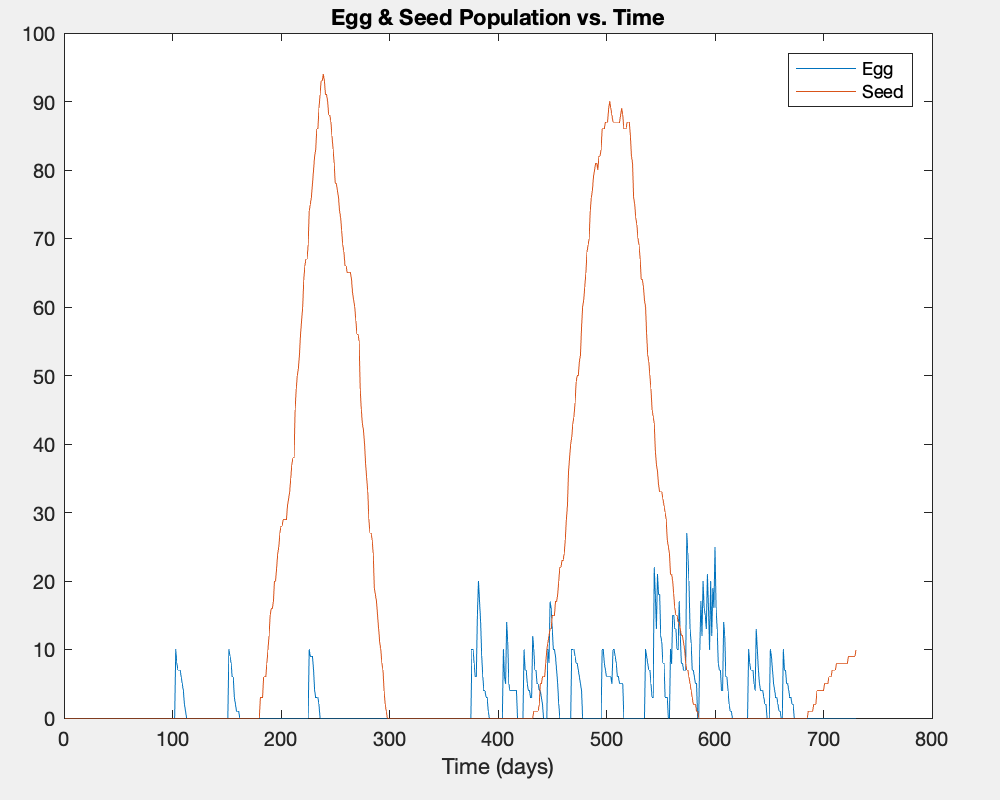
\includegraphics[width=80mm]{figures/validation_1.png} 
    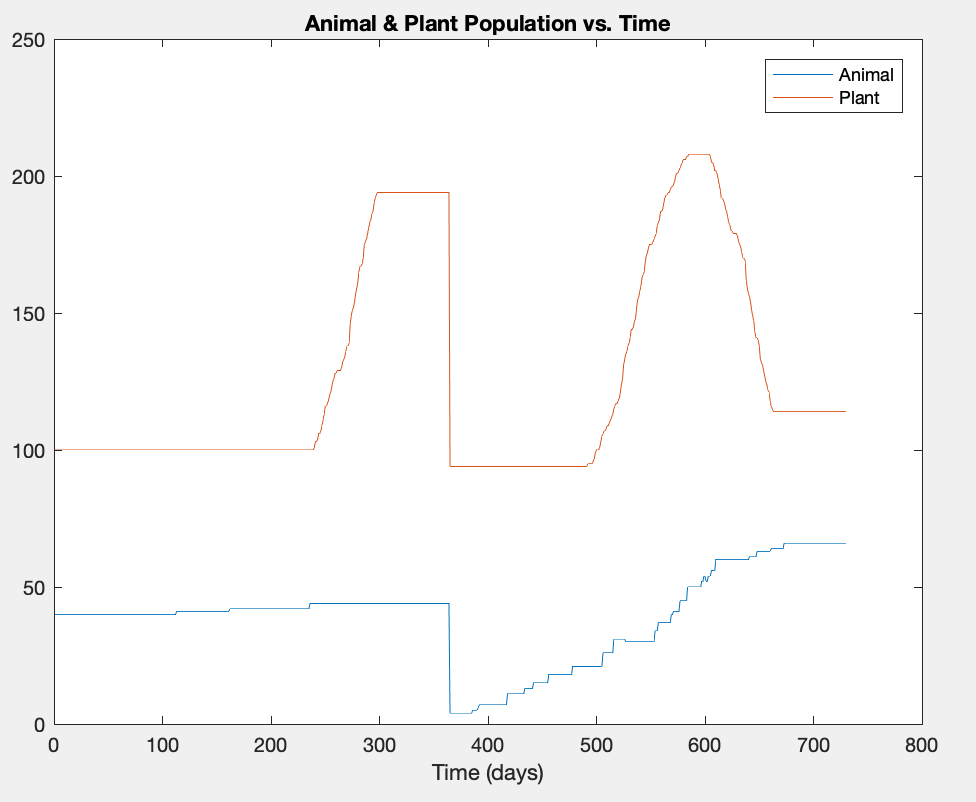
\includegraphics[width=78mm]{figures/validation_2.png}
    \caption{Population Statistics over Time}
    \end{center}
    \end{figure}

The female animals would lay 10 eggs each time, and the survival probability of eggs is $80\%$ each day. After 10 days, the eggs will become alive animals that can move freely in the environment. All animals die at age 365. The plant species can be pollinated before age 180 days, approximately half of their life span. During a following period of 120 days the plant clusters are allowed to produce seeds, dispersed through wind and with different sizes. After landing successfully, it takes 60 days for the seed to become an alive plant cluster.

From the egg and seed statistics, the modeling of egg hatching and seed growing are valid because the statistics obtained on an individual level instead of looping through the entire pollinator or plant population. The pollinator and plant populations are monotonically increasing in year one because all adult plant clusters and animals are expected to survive. At the end of year one, there are sharp declines in both species because the plant clusters and animals initialized in the model are dead (decline in animal species = initial animal population, decline in plant species = initial plant population).
\pagebreak

\subsubsection{K-means Clustering Method Explanation on Pollen Distribution}

    \begin{figure}[!htb]
    \begin{center}
    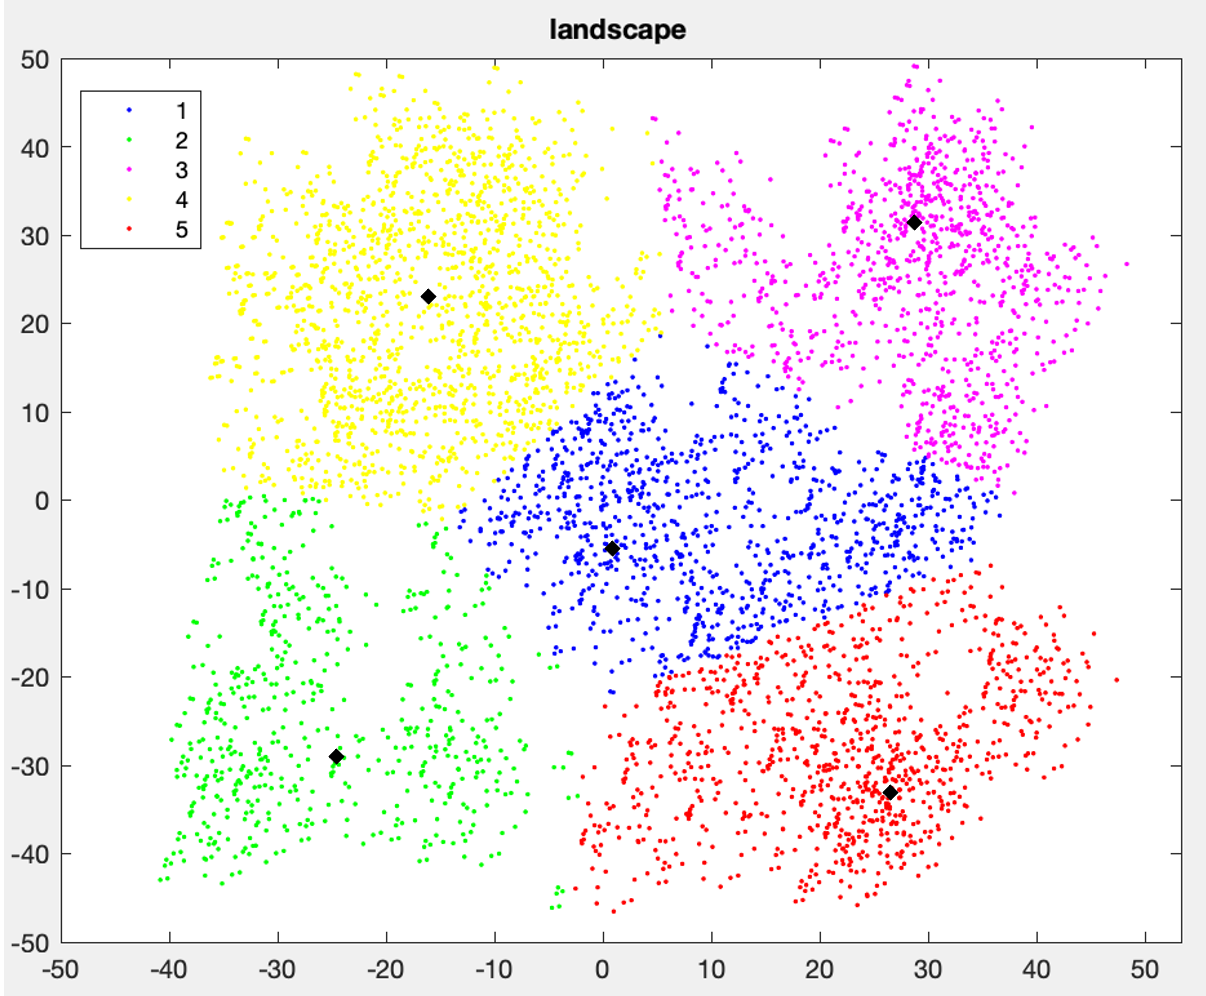
\includegraphics[width=120mm]{figures/pollen_distribution.png}
    \caption{Distribution of Pollen in the past 7 days, with 5 clustering groups}
    \end{center}
    \end{figure}
    
The above figure shows a distribution of pollen within the past 7 days, with 5 clustering groups. In the simulation, the cluster centroids are the origins considering animal movements, and the pollinators will go to a location near the pollen centroids, bounded by a factor times the scale of the landscape. Note that there is an important assumption that pollinators are not able to move as far as possible because there is a limit on how far they can move and can only pollinate a certain number of plants. At the same time, we consider that even though there might be one area in the environment that is particularly rich in pollen, not all animals will be attracted to that area. It would be  unreasonable to have pollinators move across the entire landscape within in one time step when the landscape is very large. 
\pagebreak

\section{Default Simulation Parameters}
\subsection{\textbf{Constants (User-defined)}}
\begin{table}[!htb]
\begin{tabular}{ l l }
 $max\_wind\_speed$ & 5 \\
 $max\_pollination\_success\_rate$ & 1.0 \\
 $prob\_disturb$ & 0.01 \\
\end{tabular}
\caption{\label{tab:table-name}List of Environment-related Constants}
\end{table}

\begin{table}[!htb]
\begin{tabular}{ l l }
 $num\_egg$ & 10 \\ 
 $prob\_egg\_survival$ & 0.83 \\
 $best\_temp\_egg$ & 25 \\
 $egg\_stage$ & 30 \\ 
\end{tabular}
\caption{\label{tab:table-name}List of Animal-related Constants}
\end{table}

\begin{table}[!htb]
\begin{tabular}{ l l }
 $seed\_stage$ & 60 \\ 
 $plant\_maturity\_date$ & 180 \\
 $seed\_period$ & 60 \\
 $prob\_landing$ & 0.03 \\ 
 $prob\_seed\_survival$ & 1.0 \\
 $best\_temp\_seed$ & 25 \\
 $prob\_pollen$ & 0.95 \\
\end{tabular}
\caption{\label{tab:table-name}List of Plant-related Constants}
\end{table}

\subsection{\textbf{Initial Conditions (User-defined)}}
\begin{table}[!htb]
\begin{tabular}{ l l }
 $init\_size$ & 40\\
 $init\_num\_animal$ & 20\\ 
 $init\_num\_plant$ & 100\\
 $init\_cluster\_size$ & 20 \\
 $wind\_list$ & none \\
 $temperature\_list$ & none \\
\end{tabular}
\caption{\label{tab:table-name}Initial Conditions of the Environment}
\end{table}
\end{document}
